\subsection{Simulation}
Since we have given the exact solution as:
\begin{align}
    \mathbf{u} &= \begin{pmatrix}
        x^2(1-x)^2(2y-6y^2+4y^3) \\ -y^2(1-y)^2(2x-6x^2+4x^3)
    \end{pmatrix},\\
    p &= (x(1-x)), 
\end{align}
and our boundary is defined by $\Omega = (0,1)^2$, we find, that on Omega we have:
\begin{align}
    \mathbf{u}(\Omega) &= \begin{pmatrix}
        0\\0
    \end{pmatrix}.
\end{align}

To get our system we compute local advection, stiffness and mass matrices, and assemble our global matrices for $A, G, B$.

We get the local matrices:
\begin{align}
    \frac{1}{\Delta x}\int_\Omega B_i B_k dx = \frac{1}{\Delta y}\int_\Omega B_j B_l dy &= \begin{bmatrix}
        0.5 & 0 \\
        0 & 0.5
    \end{bmatrix}\\
    \int_\Omega B_{i,x} B_k dx = \int_\Omega B_{j,y} B_l dy &=\begin{bmatrix}
        -0.5 & 0.5 \\
        -0.5 & 0.5
    \end{bmatrix}\\
    \Delta x \int_\Omega B_{i,x} B_{k,x} dx = \Delta y \int_\Omega B_{j,y} B_{l,y} dy &= \begin{bmatrix}
        1 & -1\\
        -1 & 1
    \end{bmatrix}
\end{align}

By taking the Kronecker products we can compute each product of integrals respectively. We assemble the submatrices: $A_1,A_2,G_1,G_2$, combine them as described above and take $B=-G^T$
We define our forcing term with the forcing term calculated in the exercise above. To adress the boundary conditions we manipulate the forcing term and our matrix. 

Below we show the behaviour the exact solution in \Cref{fig:streamplots}(a), and of the solution computed numerically in \Cref{fig:streamplots}(b).

\begin{figure}[H]
    \centering
    \subfigure[]{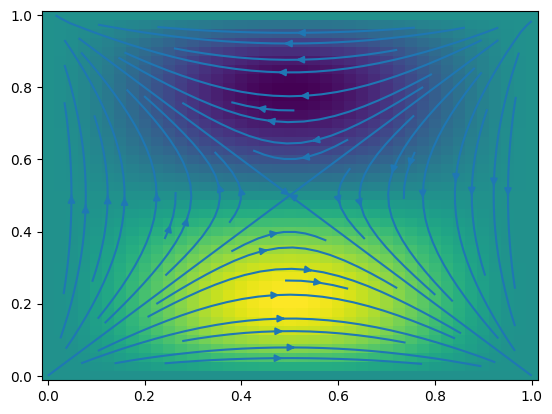
\includegraphics[width=0.45\textwidth]{Figures/Exact solution.png}}
    \hfill
    \subfigure[]{\includegraphics[width=0.45\textwidth]{Figures/Stremplot of U.png}}
    \caption{Streamplots of the (a) exact solution and of the (b) numerical solutions.}
    \label{fig:streamplots}
\end{figure}

% \begin{figure}[H]
%     \centering
%     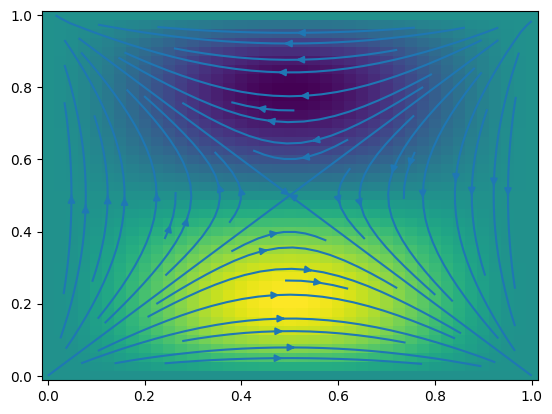
\includegraphics{Figures/Exact solution.png}
%     \caption{Exact solution}
%     \label{fig:enter-label}
% \end{figure}

% and we find compute our solutions as:
% \begin{figure}[H]
%     \centering
%     \includegraphics{Figures/Stremplot of U.png}
%     \caption{}
%     \label{fig:enter-label}
% \end{figure}

We can visualize apart the velocities and the pressure of the numerical solution respectively in \Cref{fig:velocities} and \Cref{fig:pressure} .

\begin{figure}[H]
    \centering
    \subfigure[x-component of the velocity]{\includegraphics[width=0.45\textwidth]{Figures/U1.png}}
    \hfill
    \subfigure[y-component of the velocity]{\includegraphics[width=0.45\textwidth]{Figures/U2.png}}
    \caption{Velocities of the solution computed numerically.}
    \label{fig:velocities}
\end{figure}

\begin{comment}
\begin{figure}[H]
    \centering
    \includegraphics{Figures/U1.png}
    \caption{U1}
    \label{fig:enter-label}
\end{figure}
and 
\begin{figure}[H]
    \centering
    \includegraphics{Figures/U2.png}
    \caption{U2}
    \label{fig:enter-label}
\end{figure}
\end{comment}

\begin{figure}[H]
    \centering
    \includegraphics{Figures/p.png}
    \caption{P}
    \label{fig:pressure}
\end{figure}

These plots were made for 20 cells in both directions. We see, that we do not get the exact solution. 
We do not exactly know on why this is the case. It seems to be that the matrices may be an issue. We have computed our matrices as: